\documentclass{article}

\usepackage{amsmath,amsfonts,amssymb,amsthm}
\usepackage{listings,color}
\usepackage{graphicx}


% Opening
\title{HW4 - pg147\\
Ch5 - 1-4,7}
\author{Neal D. Nesbitt}

\begin{document}
\maketitle

\theoremstyle{definition}
\newtheorem{problem}{Problem}

\lstset{basicstyle=\ttfamily,
		language=Matlab,
		keywordstyle=\bf\color{blue},
		commentstyle=\it\color{magenta},
		identifierstyle=\bf
		}

\begin{problem}

	Use bisection to determine the drag coefficient needed so that an 80 kg bungee jumper has a velocity of 36 m/s after 4 s of free fall. Note: The acceleration of gravity is 9.81 m/s\textsuperscript{2}. Start with initial guesses of $x_{l}=0.1$ and $x_{u}=0.2$ and iterate until the approximate relative error falls below 2\%. 
	
\end{problem}

We begin by reviewing the formula obtained to determine the free fall velocity of a bungee jumper:

\[ v(t) = \sqrt{\frac{gm}{c_{d}}} \tanh\left( t \sqrt{\frac{gc_{d}}{m}} \right) \]

Then we take the values as given and substitute them into the equation:

\[ v(4) = \sqrt{\frac{(9.81)(80)}{c_{d}}} \tanh\left( 4 \sqrt{\frac{(9.81)c_{d}}{80}} \right) \]

This is now a function of one variable, which we can work with. Since our methods focus on finding roots, and we wish the velocity to be 36 m/s, we subtract this value from the equation and search for a value of $c_{d}$ that gives zero overall:

\[ f(c_{d}) = v(4) - 36 = \sqrt{\frac{(9.81)(80)}{c_{d}}} \tanh\left( 4 \sqrt{\frac{(9.81)c_{d}}{80}} \right) - 36 \]

First Iteration:
\[ f(x_{l1}=0.1) = 0.8603, f(x_{u1}=0.2) = -1.1974 \]
\[ f(x_{r1}=0.15) = -0.2045 \]

Lower half contains the root since the sign changes between $x_{l}$ and $x_{r}$.\\

Second Iteration:
\[ f(x_{l2}=0.1) = 0.8603, f(x_{u2}=0.15) = -0.2045 \]
\[ f(x_{r2}=0.125) = 0.3184, \left| \varepsilon_{a} \right| = 20\% \]

Upper half contains the root.\\

Third Iteration:
\[ f(x_{l3}=0.125) = 0.3184, f(x_{u3}=0.15) = -0.2045 \]
\[ f(x_{r3}=0.1375) = 0.0546, \left| \varepsilon_{a} \right| = 9.09\% \]

Upper half contains the root.\\

Fourth Iteration:
\[ f(x_{l4}=0.1375) = 0.0546, f(x_{u4}=0.15) = -0.2045 \]
\[ f(x_{r4}=0.1437) = -0.0745, \left| \varepsilon_{a} \right| = 4.31\% \]

Lower half contains the root.\\

Fifth Iteration:
\[ f(x_{l5}=0.1375) = 0.0546, f(x_{u5}=0.1437) = -0.0745 \]
\[ f(x_{r5}=0.1406) = -0.0101, \left| \varepsilon_{a} \right| = 2.2\% \]

Lower half contains the root.\\

Sixth Iteration:
\[ f(x_{l6}=0.1375) = 0.0546, f(x_{u6}=0.1406) = -0.0101 \]
\[ f(x_{r6}=0.1391) = 0.0212, \left| \varepsilon_{a} \right| = 1.08\% \]

This completes the process with the result that $\boxed{c_{d}\approx 0.1391}$.

\begin{problem}

	Develop your own M-file for bisection in a similar fashion to Fig. 5.7. However, rather than using the maximum iterations and Eq. 5.5, employ Eq. 5.6 as your stopping criterion. Make sure to round the result of Eq. 5.6 up to the next highest integer. Test your function by solving Prob. 5.1 using $E_{a,d}=0.0001$.
	
\end{problem}

\begin{lstlisting}
function [root,fx,ea,iter] = bisectAbs(func,xl,xu,es,maxit,varargin)
% bisect: root locations
%   [root,fx,ea,iter] = bisect(func,x1,xu,es,maxit,p1,p2,...)
%       uses bisection to find a root of func 
%       within an absolute error margin
% input:
%   func = name of function
%   xl,xu = lower and upper guesses
%   es = desired absolute error (default = 0.0001)
%   maxit = maximum allowable iterations (default = 50)
%   p1,p2,... = additional parameters used by func
% output:
%   root: real root
%   fx = funtion value at root
%   ea = approximate relative error
%   iter = number of iterations

% make sure a function and upper/lower guesses were given
if nargin < 3,error('at least 3 input arguments required'),end

% make sure there is an odd number of roots within the guesses
% (hopefully only one)
test = func(xl,varargin{:})*func(xu,varargin{:});
if test > 0,error('no sign change'),end

% set default desired error and maximum iterations
if nargin < 4 | isempty(es),es=0.0001;end
if nargin < 5 | isempty(maxit),maxit=50;end

% shrink needed iterations if possible
% based on the desired absolute error
if ceil(log2(xu-xl/es)) < maxit,maxit=ceil(log2(xu-xl/es));end

% initialize iterations, root guess, and resulting error
iter = 0; xr = xl; ea = 100;
% while we have not reached the maximum iterations needed
while(1)
    % save the last root guess, and pick the new one, and step
    xrold = xr;
    xr = (xl + xu)/2;
    iter = iter + 1;
    
    % if we are not at an exact root,
    % compute the current relative error
    if xr ~= 0,ea = abs((xr - xrold)/xr)*100;end
    
    % check to see which half of the current interval
    % has an odd number of roots (hopefully just one root)
    % and set it as the new interval for the next iteration
    test = func(xl,varargin{:})*func(xr,varargin{:});
    if test < 0
        xu = xr;
    elseif test > 0
        xl = xr;
    else
        ea = 0;
    end
    
    % if we've hit the maximum number of iterations,
    % stop the loop and set the values to return
    if iter >= maxit,break,end
end
root = xr; fx = func(xr,varargin{:});
\end{lstlisting}

\begin{problem}

	Repeat Prob. 5.1, but use the false position method to obtain your solution.
	
\end{problem}

Given the same function as before, we proceed with our iterations.

\[ f(c_{d}) = v(4) - 36 = \sqrt{\frac{(9.81)(80)}{c_{d}}} \tanh\left( 4 \sqrt{\frac{(9.81)c_{d}}{80}} \right) - 36 \]

First Iteration:
\[ f(x_{l1}=0.1) = 0.8603, f(x_{u1}=0.2) = -1.1974 \]
\[ f(x_{r1}=0.1418) = -0.0352 \]

Lower half contains the root.\\

Second Iteration:
\[ f(x_{l2}=0.1) = 0.8603, f(x_{u2}=0.1418) = -0.0352 \]
\[ f(x_{r2}=0.1402) = -0.0010, \left| \varepsilon_{a} \right| = 1.14\% \]

And this completes the process with the result that $\boxed{c_{d}\approx 0.1402}$.

\begin{problem}

	Develop an M-file for the false position method. Test is by solving Prob. 5.1
	
\end{problem}

This is the exact same code as the previous example, except that the line for computing $x_{r}$ in the while loop is changed to reflect the false position algorithm.

\begin{lstlisting}
    xr = xu - func(xu)*(xl - xu)/(func(xl)-func(xu));
\end{lstlisting}

\setcounter{problem}{6}
\begin{problem}

	Determine the roots of $f(x)=-12-21x+18x^{2}-2.75x^{3}$ graphically. In addition, determine the first root of the function with bisection and false position. Use initial guesses of $x_{l}=-1$ and $x_{u}=0$ and a stopping criterion of 1\%.
	
\end{problem}

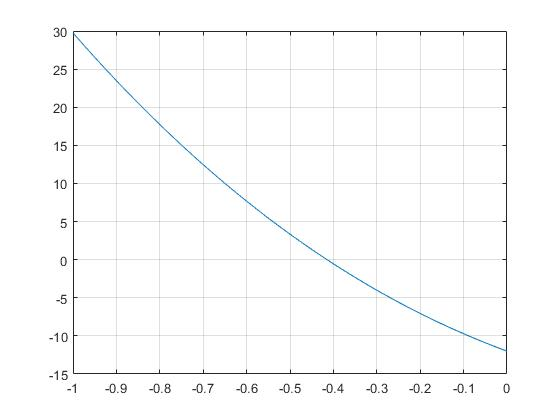
\includegraphics[width=\linewidth]{HW4-PolynomialGraph.jpg}

The graph suggests a root between -0.5 and -0.4; possibly at -0.425.\\

The bisect method calculated a root in 8 iterations at $x=-0.4180$ achieving a relative error of $\left| \varepsilon_{a} \right| =0.9346\%$ where $f(-0.4180)=0.1227$, while the false position method calculated a root in 5 iterations at $x=-0.4140$ achieving a relative error of $\left| \varepsilon_{a} \right| =0.4464\%$  where $f(-0.4140)=-0.0249$.

\end{document}